\documentclass[../../main.tex]{subfiles}

\begin{document}

\setchapterpreamble[u]{\margintoc}

\chapter{数据结构应用}

\section{栈}

栈的应用是算法中十分重要的部分。利用栈先进后出的特性,我们可以利用其历史状态解决问题。

\subsection{\href{https://leetcode-cn.com/problems/valid-parentheses/}{有效的括号}}

这个题目是栈的经典应用。我们可以利用栈来解决这个问题。我们从左到右遍历字符串,如果遇到左括号,我们就把其压入栈中,
如果遇到右括号,我们就把栈顶的元素弹出。如果弹出的左括号和当前的右括号不匹配,则说明字符串不是有效的括号组合。
如果最后栈中还有元素,那么说明字符串不是有效的括号组合。

\lstinputlisting[language=C++]{code/valid-parentheses.cpp}

\subsection{\href{https://leetcode-cn.com/problems/evaluate-reverse-polish-notation/}{逆波兰表达式求值}}

首先我们必须去理解逆波兰表达式的含义。例如,对于表达式\texttt{["2", "1", "+", "3", "*"]},其含义为
\texttt{(2 + 1) * 3 = 9}。我们可以利用栈来解决这个问题。很显然我们可以很简单地用递归的方式去解决这个
问题,我们从右到左遍历表达式,如果我们遇到运算符,证明我们需要递归地求解左右两边的表达式。当遇到数字时,
我们直接返回这个数字。

\lstinputlisting[language=C++]{code/evaluate-reverse-polish-notation-recursive.cpp}

既然能用递归实现,那么也能够用栈实现,实际上用栈实现才是普遍做法吧,可以看见,我们可以把数字压栈,当我们遇到了
一个新的运算符时,我们就从栈中弹出两个数字,然后进行运算,然后把结果压栈。最后栈中只会剩下一个数字。然后不断
进行这个数字,最后返回栈顶的数字即可。

\lstinputlisting[language=C++]{code/evaluate-reverse-polish-notation-stack.cpp}

\section{单调栈}

单调栈是栈的一个重要应用,其可以用于解决一些问题。单调栈的特点是栈中的元素是单调递增或者单调递减的。我们可以利用
单调栈来解决一些问题。

\subsection{\href{https://leetcode.cn/problems/daily-temperatures/}{每日温度}}

本质上,我们需要找到每个元素右边第一个比它大的元素。我们可以利用单调栈来解决这个问题。我们这个栈维持单调递减的
顺序,当遇到了一个新的元素,我们从栈中弹出所有比这个元素小的元素,然后把这个元素压栈。这样,我们就可以找到每个
元素右边第一个比它大的元素\sidenote{
这样讲可能仍然抽象了,我们举一个例子来说明这个问题。假设我们有一个数组\texttt{[73, 74, 75, 71, 69, 72, 76, 73]}。
我们维护一个单调递减的栈,我们从左到右遍历数组,当我们遇到73时,我们把其压栈,当我们遇到74时,
我们把73弹出,然后把74压栈。当我们遇到75时,我们把74弹出,
然后把75压栈。当我们遇到\texttt{71}时,然后把71压栈。当我们遇到69时,继续把69压栈。当我们遇到72时,
我们弹出69,71,然后把72压栈。当我们遇到76时,我们弹出75然后把76压栈。当我们遇到73时,我们把
73压栈。这样我们就找到了每个元素右边第一个比它大的元素。
}。

\lstinputlisting[language=C++]{code/daily-temperatures.cpp}

\begin{kaobox}[title=类似题目]
  \begin{itemize}
    \item \href{https://leetcode-cn.com/problems/next-greater-element-i/}{下一个更大元素 I}
    \item \href{https://leetcode-cn.com/problems/next-greater-element-ii/}{下一个更大元素 II}
    \item \href{https://leetcode-cn.com/problems/next-greater-node-in-linked-list/}{链表中的下一个更大节点}
    \item \href{https://leetcode.cn/problems/remove-nodes-from-linked-list/}{从链表中移除节点}
  \end{itemize}
\end{kaobox}

\subsection{\href{https://leetcode.cn/problems/trapping-rain-water/}{接雨水}}

接雨水是一个相当复杂的题目,我们必须从最原始的角度去思考问题,最终不断优化我们的问题,从而解决该题。首先我们
需要思考,如何才能接到雨水。显然,按照正常人的思维,我们知道必须两边要有墙,如下图所示:

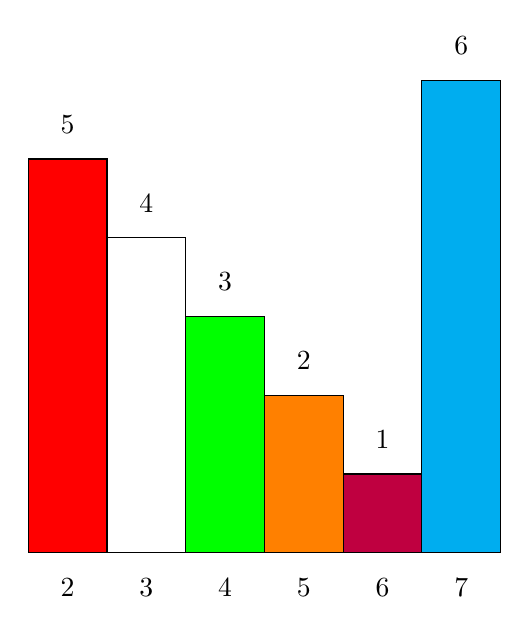
\begin{tikzpicture}
  \draw[fill=red] (1,5) rectangle (2,0);
  \draw[fill=white] (2,4) rectangle (3,0);
  \draw[fill=green] (3,3) rectangle (4,0);
  \draw[fill=orange] (4,2) rectangle (5,0);
  \draw[fill=purple] (5,1) rectangle (6,0);
  \draw[fill=cyan] (6,6) rectangle (7,0);

  \foreach \x/\y in {2/5,3/4,4/3,5/2,6/1,7/6} {
      \draw (\x-0.5,-0.2) node[below] {\x};
      \draw (\x-0.5,\y+0.2) node[above] {\y};
  }
\end{tikzpicture}

在下图中,对于$x = 3$,我们需要找到其左侧和右侧的比当前值大的最近的值,即$x = 1$和$x = 7$。
然后我们就可以计算$x = 2$能够容纳的雨水量。对于每一个$x$,我们都需要找到其左侧和右侧的比当前值大的最近的值。
然而,你马上就会发现这样做的弊端,对于$x = 3, 4, 5, 6$实际上我们都在做重复的工作,我们都需要找到$x = 1$
和$x = 7$,这是我们需要优化的点,我们首先给出暴力的解法。

\lstinputlisting[language=C++]{code/trapping-rain-water-brute-force.cpp}

我们其实已经给出了优化的思路。就是我们会做出许多重复的计算。我们思考一下我能够记录下来一些信息,从而避免重复
的计算吗?答案是肯定的。我们可以在计算之前,就把左侧和右侧的比当前值大的最近的值记录下来。这样我们就可以在循环
中使用这些信息,从而避免重复的计算。

\lstinputlisting[language=C++]{code/trapping-rain-memozied.cpp}

但是,我们是不是应该换一个思维来处理这个问题了。我们按照递减的顺序维持一个单调栈,当我们遇到一个新的元素时,
如果这个元素比栈顶元素大,那么我们可能遇到了一个坑,我们可以计算这个坑的大小。实际上,我们此时采用的思路
就变为了按照行来计算水坑的大小,如下图所示:

\begin{tikzpicture}
  \draw[fill=red] (1,5) rectangle (2,0);
  \draw[fill=white] (2,4) rectangle (3,0);
  \draw[fill=green] (3,3) rectangle (4,0);
  \draw[fill=orange] (4,2) rectangle (5,0);
  \draw[fill=purple] (5,1) rectangle (6,0);
  \draw[fill=cyan] (6,6) rectangle (7,0);

  \foreach \x/\y in {2/5,3/4,4/3,5/2,6/1,7/6} {
      \draw (\x-0.5,-0.2) node[below] {\x};
      \draw (\x-0.5,\y+0.2) node[above] {\y};
  }

  \draw [fill=blue](5,1) rectangle (6,2);
  \draw [arrow, color=red] (5, 1.5) -- (6, 1.5);

  \draw [fill=blue](4,2) rectangle (6,3);
  \draw [arrow, color=red] (4, 2.5) -- (6, 2.5);

  \draw [fill=blue](3,3) rectangle (6,4);
  \draw [arrow, color=red] (3, 3.5) -- (6, 3.5);

  \draw [fill=blue](2,4) rectangle (6,5);
  \draw [arrow, color=red] (2, 4.5) -- (6, 4.5);

\end{tikzpicture}

从而,我们就能给出如下的代码。我们可以发现栈顶元素永远是当前元素,其上一个入栈的元素是第一个大于当前元素的元素。
如果我们遇到了一个比栈顶元素大的元素,那么就证明我们发现了当前栈顶元素的左侧第一个比它大的元素,以及右侧第一个比它
大的元素,这就与我们的暴力解法相统一了。

\lstinputlisting[language=C++]{code/trapping-rain-water-stack.cpp}

\subsection{\href{https://leetcode-cn.com/problems/largest-rectangle-in-histogram/}{柱状图中最大的矩形}}

解决这个问题首先必须要明确什么时候矩形是最大的。很明显我们希望这个矩形尽可能越宽,同时尽可能越高。所以
这个问题的暴力方法就出来了。我们需要找每个柱子左右两边第一个小于该柱子的柱子。

那么按照接雨水的方法,我们可以再次设置一个单调递增的栈。利用接雨水的方法解决这个问题。

\lstinputlisting[language=C++]{code/largest-rectangle-in-histogram.cpp}

\end{document}
